
\documentclass[12pt, letterpaper]{article}

% ── Codificación y lenguaje ──────────────────────────────────
\usepackage[utf8]{inputenc}
\usepackage[T1]{fontenc}
\usepackage[spanish]{babel}


% ── Márgenes ─────────────────────────────────────────────────
\usepackage[top=2.5cm, bottom=2.5cm, left=3cm, right=3cm]{geometry}

% ── Matemáticas ──────────────────────────────────────────────
\usepackage{amsmath, amssymb, amsthm}

% ── Expresiones regulares y verbatim elegante ────────────────
\usepackage{listings}           % bloques de código / regex
\usepackage{xcolor}             % colores para listings

% ── Tablas y figuras ─────────────────────────────────────────
\usepackage{booktabs}
\usepackage{array}
\usepackage{float}
\usepackage{graphicx} % en el preámbulo


% ── Hipervínculos ────────────────────────────────────────────
\usepackage{hyperref}
\hypersetup{
    colorlinks = true,
    linkcolor  = blue!60!black,
    urlcolor   = blue!60!black,
}


% ── Encabezado y pie de página ───────────────────────────────
\usepackage{fancyhdr}
\usepackage{longtable}
\setlength{\headheight}{15pt}
\pagestyle{fancy}
\fancyhf{}
\lhead{\textsc{Compiladores}}
\rhead{\textsc{Patito — Entrega \#5}}
\cfoot{\thepage}

% ── Ambientes de teoremas ────────────────────────────────────
\theoremstyle{definition}
\newtheorem{definicion}{Definición}[section]
\newtheorem{ejemplo}{Ejemplo}[section]
\newtheorem{regla}{Regla}[section]

% ── Estilo de listings para expresiones regulares / código ───
\lstdefinestyle{regex}{
    basicstyle    = \ttfamily\small,
    keywordstyle  = \color{blue!70!black}\bfseries,
    commentstyle  = \color{green!50!black}\itshape,
    stringstyle   = \color{orange!80!black},
    backgroundcolor = \color{gray!8},
    frame         = single,
    framerule     = 0.4pt,
    rulecolor     = \color{gray!40},
    breaklines    = true,
    captionpos    = b,
    numbers       = left,
    numberstyle   = \tiny\color{gray},
    stepnumber    = 1,
    numbersep     = 6pt,
    showstringspaces = false,
    tabsize       = 4,
}

% Macro para escribir una regex en línea con formato
\newcommand{\rx}[1]{\texttt{\textcolor{blue!70!black}{#1}}}

% Macro para símbolo de producción en gramáticas
\newcommand{\produce}{\;\longrightarrow\;}
\newcommand{\OR}{\;\mid\;}

% ============================================================
\begin{document}

% ── Portada ──────────────────────────────────────────────────
\begin{titlepage}
    \centering
    \vspace*{2cm}
    {\LARGE\bfseries Compiladores\par}
    \vspace{0.5cm}
    {\large Patito - entrega \#5 \par}
    \vspace{2cm}
    {\large Carlos Fernando Ramos Mena\par}
    \vspace{0.3cm}
    {\normalsize Matrícula: A01197622\par}
    \vspace{0.5cm}
    {\normalsize Tec de Monterrey\par}
    \vfill
    {\normalsize \today\par}
\end{titlepage}


% ============================================================
\section{Introducción}
% ============================================================
A continuación se adjuntan las bases incluidas en el entregable 0 mismas que serán usadas en próximos entregables.


% ============================================================
\section{Definición de Tokens }
% ============================================================

\begin{center}
\begin{longtable}{|p{3.5cm}|p{5.5cm}|p{5cm}|}
    \hline
    \texttt{Token} & \texttt{Significado} & \texttt{Regex} \\
    \hline
    \endfirsthead

    \multicolumn{3}{r}{\small\textit{(continúa de la página anterior)}} \\
    \hline
    \texttt{Token} & \texttt{Significado} & \texttt{Regex} \\
    \hline
    \endhead

    \hline
    \multicolumn{3}{r}{\small\textit{(continúa en la siguiente página)}} \\
    \endfoot

    \hline
    \endlastfoot

    %PALABRAS RESERVADAS
    \texttt{TOKEN\_PROGRAM}    & Indica inicio de un programa         & \rx{PROGRAM} \\ \hline
    \texttt{TOKEN\_START}      & Indica el inicio de un cuerpo        & \rx{BEGIN}    \\ \hline
    \texttt{TOKEN\_END}        & Indica el fin de un cuerpo           & \rx{END}      \\ \hline
    \texttt{TOKEN\_VARS}       & Indica el inicio de una variable     & \rx{VAR}      \\ \hline
    \texttt{TOKEN\_INT}        & Tipo entero                          & \rx{INT}      \\ \hline
    \texttt{TOKEN\_FLOAT}      & Tipo flotante                        & \rx{FLOAT}    \\ \hline
    \texttt{TOKEN\_PRINT}      & Indica inicio de impresión           & \rx{PRINT}    \\ \hline
    \texttt{TOKEN\_WHILE}      & Indica inicio de ciclo               & \rx{WHILE}    \\ \hline
    \texttt{TOKEN\_DO}         & Indica inicio del cuerpo de un ciclo & \rx{DO}       \\ \hline
    \texttt{TOKEN\_IF}         & Indica inicio de un condicional      & \rx{IF}       \\ \hline
    \texttt{TOKEN\_ELSE}       & Indica inicio de condicional else    & \rx{ELSE}     \\ \hline
    \texttt{TOKEN\_VOID}       & Retorno nulo de una función          & \rx{VOID}     \\ \hline
    \texttt{TOKEN\_RETURN}     & Retorno de una función               & \rx{RETURN}   \\ \hline

    %REGEX
    \texttt{TOKEN\_ID}         & Identificador                        & \rx{[a-zA-Z\_][a-zA-Z0-9\_]*} \\ \hline
    \texttt{TOKEN\_LETRERO}    & Letrero a imprimir en PRINT & \rx{\textquotedbl[\textasciicircum\textquotedbl]*\textquotedbl}\\ \hline    
    \texttt{TOKEN\_CTE\_INT}   & Constante entera                     & \rx{[0-9]+}       \\ \hline
    \texttt{TOKEN\_CTE\_FLOAT} & Constante flotante                   & \rx{[0-9]+.[0-9]+}\\ \hline
    %PUNTUACION
    \texttt{TOKEN\_SEMICOLON}  & Terminación de instrucción           & \rx{;}            \\ \hline
    \texttt{TOKEN\_COMMA}      & Separador de continuidad             & \rx{,}            \\ \hline
    \texttt{TOKEN\_COLON}      & Definición                           & \rx{:}            \\ \hline
    \texttt{TOKEN\_LBRACE}     & Inicio de bloque                     & \rx{\{}           \\ \hline
    \texttt{TOKEN\_RBRACE}     & Fin de bloque                        & \rx{\}}           \\ \hline
    \texttt{TOKEN\_LBRACKET}   & Inicio de delimitación               & \rx{[}            \\ \hline
    \texttt{TOKEN\_RBRACKET}   & Fin de delimitación                  & \rx{]}            \\ \hline
    \texttt{TOKEN\_LPAREN}     & Inicio de paréntesis                 & \rx{(}            \\ \hline
    \texttt{TOKEN\_RPAREN}     & Fin de paréntesis                    & \rx{)}            \\ \hline
    %OPERADORES
    \texttt{TOKEN\_SUM}        & Suma                                 & \rx{+}            \\ \hline
    \texttt{TOKEN\_SUBS}      & Resta                                & \rx{-}            \\ \hline
    \texttt{TOKEN\_DIV}        & División                             & \rx{/}            \\ \hline
    \texttt{TOKEN\_TIMES}      & Multiplicación                       & \rx{*}            \\ \hline
    \texttt{TOKEN\_EQUALS}     & Asignación                           & \rx{=}            \\ \hline
    \texttt{TOKEN\_GT}         & Mayor que                            & \rx{\textgreater} \\ \hline
    \texttt{TOKEN\_LT}         & Menor que                            & \rx{\textless}    \\ \hline
    \texttt{TOKEN\_DIFF}       & Diferente                            & \rx{!=}           \\ \hline
    \texttt{TOKEN\_ISEQUAL}    & Comparación de igualdad              & \rx{==}           \\ \hline

\end{longtable}
\end{center}

% ── 2.3 Comentarios y espacios en blanco ─────────────────────
\subsection{Espacios en Blanco y Comentarios}

Los espacios en blanco y comentarios son reconocidos pero \emph{descartados}
por el analizador léxico (no generan token):

\begin{center}
\begin{longtable}{|p{3.5cm}|p{5.5cm}|p{5cm}|}
    \caption{Patrones descartados} \\
    \hline
    \texttt{Patrón} & \texttt{Regex} & \texttt{Nota} \\
    \hline
    \endfirsthead
    \hline
    \texttt{Patrón} & \texttt{Regex} & \texttt{Nota} \\
    \hline
    \endhead
    \hline
    \endfoot
    \hline
    \endlastfoot

    \texttt{ESPACIO}      & \rx{[ \textbackslash t\textbackslash n\textbackslash r]+}      & Se ignora \\ \hline
    \texttt{COMENTARIO}   & \rx{//[\textasciicircum\textbackslash n]*}                     & Comentario de línea \\ \hline
    \texttt{COMENTARIO}   & \rx{/\textbackslash*[\textbackslash s\textbackslash S]*?\textbackslash*/} & Comentario de bloque \\ \hline

\end{longtable}
\end{center}

% ============================================================
\section{Gramática Libre de Contexto}
% ============================================================


\begin{itemize}
    \item El conjunto de no terminales es:
    \begin{multline*}
        V = \{\, \mathit{PROGRAMA},\; \mathit{VARS},\; \mathit{FUNCS},\;
                 \mathit{CUERPO},\; \mathit{TIPO},\; \mathit{ESTATUTO},\; \\
                 \mathit{EXPRESION},\; \mathit{EXP},\; \mathit{LLAMADA},\;
                 \mathit{TERMINO},\; \mathit{FACTOR},\; \mathit{IMPRIME},\; \\
                 \mathit{CICLO},\; \mathit{ASIGNA},\; \mathit{CONDICION},\;
                 \mathit{CTE} \,\}
    \end{multline*} 
    \item El conjunto de terminales es:
    \begin{multline*}
        \Sigma = \{\,
                 \texttt{TOKEN\_PROGRAM},\; \texttt{TOKEN\_START},\;
                 \texttt{TOKEN\_END},\; \texttt{TOKEN\_VARS},\; \\
                 \texttt{TOKEN\_INT},\; \texttt{TOKEN\_FLOAT},\;
                 \texttt{TOKEN\_PRINT},\; \texttt{TOKEN\_WHILE},\;
                 \texttt{TOKEN\_DO},\; \texttt{TOKEN\_IF},\; \\
                 \texttt{TOKEN\_ELSE},\; \texttt{TOKEN\_VOID},\; \texttt{TOKEN\_RETURN},\;
                 \texttt{TOKEN\_ID},\; \texttt{TOKEN\_LETRERO},\; \\
                 \texttt{TOKEN\_CTE\_INT},\; \texttt{TOKEN\_CTE\_FLOAT},\;
                 \texttt{TOKEN\_COLON}, \texttt{TOKEN\_SEMICOLON},\; \texttt{TOKEN\_COMMA},\; \\
                 \texttt{TOKEN\_LBRACE},\; \texttt{TOKEN\_RBRACE},\;
                 \texttt{TOKEN\_LPAREN},\; \texttt{TOKEN\_RPAREN},\; \\
                 \texttt{TOKEN\_SUM},\; \texttt{TOKEN\_SUBS},\;
                 \texttt{TOKEN\_TIMES},\; \texttt{TOKEN\_DIV},\; \\
                 \texttt{TOKEN\_EQUALS},\; \texttt{TOKEN\_GT},\;
                 \texttt{TOKEN\_LT},\; \texttt{TOKEN\_DIFF},\;
                 \texttt{TOKEN\_ISEQUAL} \,\}
    \end{multline*} 

    \item $P$ es el conjunto de \emph{producciones}  

    \item $S = \mathit{PROGRAMA}$ es el \emph{símbolo inicial}.
\end{itemize}

\subsection{Producciones}


{\small
\begin{align}
    % CTE y TIPO
    \mathit{CTE} &\produce \texttt{TOKEN\_CTE\_INT} \OR \texttt{TOKEN\_CTE\_FLOAT} \label{p:cte} \\[3pt]
    \mathit{TIPO} &\produce \texttt{TOKEN\_INT} \OR \texttt{TOKEN\_FLOAT} \label{p:tipo} \\[3pt]
    % FACTOR
    \mathit{FACTOR} &\produce \texttt{TOKEN\_LPAREN}\;\mathit{EXPRESION}\;\texttt{TOKEN\_RPAREN} \\        
    & \OR \texttt{TOKEN\_SUM}\; \mathit{FACTOR'} \nonumber \\
    & \OR \texttt{TOKEN\_SUBS}\;  \mathit{FACTOR'} \nonumber \\
    & \OR \mathit{FACTOR'} \nonumber \\           
    & \OR \mathit{LLAMADA} \nonumber \label{p:factor}  \\[3pt]   
    \mathit{FACTOR'} & \produce  \mathit{CTE}  \\
                    & \OR \texttt{TOKEN\_ID} \nonumber \\[3pt]  
    % LLAMADA
    \mathit{LLAMADA} &\produce \texttt{TOKEN\_ID}\;\texttt{TOKEN\_LPAREN}\;%
                       \mathit{LLAMADA'}\;\texttt{TOKEN\_RPAREN} \\[3pt]
    \mathit{LLAMADA'} &\produce  \mathit{EXPRESION}\; \mathit{LLAMADA''} \\                     
                      & \OR \varepsilon \nonumber \\[3pt]      
    \mathit{LLAMADA''} &\produce  \texttt{TOKEN\_COMMA} \; \mathit{EXPRESION}  \; \mathit{LLAMADA''}   \\                     
                      & \OR  \varepsilon \; \;  \nonumber\\[3pt]                                           
    % TÉRMINO
    \mathit{TERMINO} &\produce \mathit{FACTOR} \;  \mathit{TERMINO'}\;  \\[3pt]
    % TÉRMINO'
    \mathit{TERMINO'} & \produce \texttt{TOKEN\_TIMES} \; \mathit{TERMINO}\\
                    & \OR \texttt{TOKEN\_DIV} \; \mathit{TERMINO}  \nonumber \\ 
                    & \OR \varepsilon  \nonumber \\[3pt]
    % EXP
    \mathit{EXP} &\produce \mathit{TERMINO} \; \mathit{EXP'} \label{p:exp}  \\[3pt]
    % EXP'
    \mathit{EXP'} & \produce \texttt{TOKEN\_SUM} \; \mathit{EXP}\\
                    & \OR \texttt{TOKEN\_SUBS} \; \mathit{EXP}  \nonumber\\                    
                    & \OR \varepsilon  \nonumber\\[3pt]  
    % EXPRESIÓN
    \mathit{EXPRESION} &\produce \mathit{EXP}\; \mathit{EXPRESION'}\; \\[3pt]   
    % EXPRESIÓN
    \mathit{EXPRESION'} &\produce \mathit{EXPRESION''} \\
                       & \OR \varepsilon   \nonumber \\[3pt]  
    % EXPRESIÓN'
    \mathit{EXPRESION''} &\produce \texttt{TOKEN\_GT}\; \mathit{EXP} \\
                        & \OR \texttt{TOKEN\_LT}\; \mathit{EXP} \nonumber \\
                        & \OR \texttt{TOKEN\_DIFF}\; \mathit{EXP}  \nonumber \\
                        & \OR \texttt{TOKEN\_ISEQUAL}\; \mathit{EXP} \nonumber  \\ \nonumber
\end{align}}
\small{
    \begin{align}
    % ASIGNA
    \mathit{ASIGNA} &\produce \texttt{TOKEN\_ID}\;\texttt{TOKEN\_EQUALS}\;%
    \mathit{EXPRESION}\;\texttt{TOKEN\_SEMICOLON}  \\[3pt]
    % IMPRIME
    \mathit{IMPRIME} &\produce \texttt{TOKEN\_PRINT}\;\texttt{TOKEN\_LPAREN}\;%
                    \mathit{IMPRIME'}\;\texttt{TOKEN\_RPAREN}\;\texttt{TOKEN\_SEMICOLON}\\[3pt]
    % IMPRIME''
    \mathit{IMPRIME'} &\produce \mathit{EXPRESION}\; \mathit{IMPRIME''} \\
                       & \OR \texttt{TOKEN\_LETRERO}\; \mathit{IMPRIME''}  \nonumber \\[3pt]
    % IMPRIME'
    \mathit{IMPRIME''} &\produce \texttt{TOKEN\_COMMA}\; \mathit{IMPRIME'} \\
                       & \OR \varepsilon  \nonumber \\[3pt]
    % CONDICIÓN
    \mathit{CONDICION} &\produce \texttt{TOKEN\_IF}\;\texttt{TOKEN\_LPAREN}\;%
                                  \mathit{EXPRESION}\;\texttt{TOKEN\_RPAREN} \ \\
                         &\phantom{{}\produce{}}% 
                           \mathit{CUERPO}\; \mathit{CONDICION'}\; \texttt{TOKEN\_SEMICOLON}\; \nonumber \label{p:condicion} \\[3pt]
    % CONDICIÓN'
    \mathit{CONDICION'} &\produce \OR  \texttt{TOKEN\_ELSE}\; \mathit{CUERPO}\; \\ 
    & \OR \varepsilon \nonumber \\[3pt]
    % CICLO
    \mathit{CICLO} &\produce \texttt{TOKEN\_WHILE}\;\texttt{TOKEN\_LPAREN}\;%
                              \mathit{EXPRESION}\;\texttt{TOKEN\_RPAREN}  \\
                   &\phantom{{}\produce{}}%
                      \texttt{TOKEN\_DO}\;\mathit{CUERPO}\; \texttt{TOKEN\_SEMICOLON} \nonumber \label{p:ciclo} \\[3pt]
    % ESTATUTO
    \mathit{ESTATUTO} &\produce \mathit{ASIGNA} \\
                      & \OR \mathit{CONDICION} \nonumber\\
                      & \OR \mathit{CICLO} \nonumber \\
                      &\OR \mathit{IMPRIME} \nonumber\\
                      & \OR \mathit{LLAMADA}\;\texttt{TOKEN\_SEMICOLON} \nonumber\\
                      & \OR  \texttt{TOKEN\_LBRACKET}\;\mathit{ESTATUTO'}\; \texttt{TOKEN\_RBRACKET}\nonumber \\[3pt]
    % ESTATUTO
    \mathit{ESTATUTO'} &\produce \mathit{ESTATUTO}\; \mathit{ESTATUTO'} \\
                      & \OR \varepsilon \nonumber \\[3pt]                                            
    % VARS
    \mathit{VARS} &\produce \texttt{TOKEN\_VARS}\; \mathit{VARS'}\;  \\[3pt]
    %VARS'
    \mathit{VARS'} &\produce \texttt{TOKEN\_ID}\; \mathit{VARS''}\; \mathit{TIPO}\;\texttt{TOKEN\_SEMICOLON}\;  \mathit{VARS'''} \\[3pt]
    %VARS''
    \mathit{VARS''}  &\produce \texttt{TOKEN\_COMMA}\; \texttt{TOKEN\_ID}\; \mathit{VARS''}\\
                     &\OR \texttt{TOKEN\_COLON} \nonumber\\[3pt]
    %VARS'''
    \mathit{VARS'''}  &\produce \mathit{VARS'}\\
                     &\OR \varepsilon \nonumber \\[3pt]    
    % CUERPO
    \mathit{CUERPO} &\produce  \texttt{TOKEN\_LBRACE}\; \mathit{CUERPO'} \; \texttt{TOKEN\_RBRACE}\; \\[3pt]
    % CUERPO'
    \mathit{CUERPO'} &\produce \mathit{ESTATUTO} \;\mathit{CUERPO'} \\ 
                     & \OR \varepsilon \nonumber\\[3pt]
    % FUNCS
    \mathit{FUNCS} &\produce \texttt{TOKEN\_VOID}\; \texttt{TOKEN\_ID}\;\texttt{TOKEN\_LPAREN}\;  \mathit{FUNC'}\; 
                    \texttt{TOKEN\_RPAREN}\; \\ 
                   &\texttt{TOKEN\_LBRACE} \; \mathit{FUNC'''} \;
                     \mathit{CUERPO} \; \mathit{FUNCS''''} \;   \texttt{TOKEN\_RBRACE} \; \texttt{TOKEN\_SEMICOLON} \; \nonumber\\
                   &\OR{}  \mathit{TIPO}\; \texttt{TOKEN\_ID}\;\texttt{TOKEN\_LPAREN}\;  \mathit{FUNC'}\; 
                    \texttt{TOKEN\_RPAREN}\; \nonumber\\
                   &\texttt{TOKEN\_LBRACE} \; \mathit{FUNC'''} \;
                     \mathit{CUERPO} \;  \mathit{FUNCS''''} \;  \texttt{TOKEN\_RBRACE} \; \texttt{TOKEN\_SEMICOLON} \; \nonumber\\[3pt]
    % FUNCS'
    \mathit{FUNCS'} &\produce \texttt{TOKEN\_ID}\;\texttt{TOKEN\_COLON}\;\mathit{TIPO}\; \mathit{FUNC''}\;  \\
                   & \OR \varepsilon \nonumber \\[3pt] \nonumber
\end{align}

}
\small{
    \begin{align}
    % FUNCS''
    \mathit{FUNCS''} &\produce \texttt{TOKEN\_COMMA}\; \texttt{TOKEN\_ID}\;\texttt{TOKEN\_COLON}\;\mathit{TIPO}\; \mathit{FUNC''}\;  \\
                   & \OR \varepsilon \nonumber\\[3pt]
    % FUNCS'''
    \mathit{FUNCS'''} &\produce \texttt{TOKEN\_VARS}\;  \\
                   & \OR \varepsilon \nonumber\\[3pt]
    % FUNCS''''
    \mathit{FUNCS''''} &\produce \texttt{TOKEN\_RETURN}\; \mathit{EXPRESION}\;\texttt{TOKEN\_SEMICOLON}\; \\
                    & \OR \varepsilon \nonumber\\[3pt]
    % PROGRAMA
    \mathit{PROGRAMA} &\produce \texttt{TOKEN\_PROGRAM}\;\texttt{TOKEN\_ID}\;%
                                 \texttt{TOKEN\_SEMICOLON}\;\mathit{PROGRAMA'}\;\mathit{PROGRAMA''}\   \\
                      &\phantom{{}\produce{}}%
                         \texttt{TOKEN\_START}\;\mathit{CUERPO}\;\texttt{TOKEN\_END} \nonumber\\[3pt]
    % PROGRAMA'
    \mathit{PROGRAMA'} &\produce \mathit{VARS} \\
                      &\OR \varepsilon  \nonumber\\[3pt]
    % PROGRAMA'
    \mathit{PROGRAMA''} &\produce \mathit{FUNCS}\; \mathit{FPROGRAMA''}  \\
                      &\OR \varepsilon  \nonumber\\[3pt]\nonumber
    \end{align}
}

\section{Léxico y Sintaxis}
% ============================================================
Como parte de esta sección llevé a cabo una investigación de distintas herramientas automáticas de Scanners y Parsers.

A continuación se presentan los resultados de esta investigación.

\begin{center}
\begin{longtable}{|p{3.5cm}|p{11cm}|}
    \caption{Analísis de Yacc} \\
    \hline
    \multicolumn{2}{|l|}{    \texttt{Lex \& Yacc}     } \\
    \hline
    \texttt{Evaluación} & \texttt{Nota} \\
    \hline
    \endfirsthead
    \hline
    \endfoot
    \hline
    \endlastfoot
    \hline
    \texttt{Plataforma y lenguaje base}      & \texttt{C, cross platform}   \\ \hline
    \texttt{Formato requerido en las entradas}   & \texttt{Hay dos declaraciones, en C y en LEX. Las importantes son en C y en LEX se definen regex y simbolos}                  \\ \hline
    \texttt{Tipo de ejecución}   & \texttt{YACC crea el parser, y crea los tokens del LEX después lo traslada a C} \\ \hline
    \texttt{Tipo de licenciamiento}   & \texttt{MIT License, gratis} \\ \hline
    \texttt{Herramientas teóricas en las quese basan}   & \texttt{Expresiones regulares y gramática libre de contexto} \\ \hline

\end{longtable}
\end{center}

\begin{center}
\begin{longtable}{|p{3.5cm}|p{11cm}|}
    \caption{Análisis de Lark} \\
    \hline
    \multicolumn{2}{|l|}{    \texttt{Lark}     } \\
    \hline
    \texttt{Evaluación} & \texttt{Nota} \\
    \hline
    \endfirsthead
    \hline
    \endfoot
    \hline
    \endlastfoot
    \hline
    \texttt{Plataforma y lenguaje base}      & \texttt{python}   \\ \hline
    \texttt{Formato requerido en las entradas}   & \texttt{Utiliza string de Python y archivos .lark}  \\ \hline
    \texttt{Tipo de ejecución}   & \texttt{Construye un árbol en base a la gramática AST, ejecución embedida} \\ \hline
    \texttt{Tipo de licenciamiento}   & \texttt{MIT License, gratis} \\ \hline
    \texttt{Herramientas teóricas en las quese basan}   & \texttt{Expresiones regulares, LARL EARLEY y CYK} \\ \hline
\end{longtable}
\end{center}


\begin{center}
\begin{longtable}{|p{3.5cm}|p{11cm}|}
    \caption{Análisis de LALRPOP} \\
    \hline
    \multicolumn{2}{|l|}{    \texttt{LALRPOP}     } \\
    \hline
    \texttt{Evaluación} & \texttt{Nota} \\
    \hline
    \endfirsthead
    \hline
    \endfoot
    \hline
    \endlastfoot
    \hline
    \texttt{Plataforma y lenguaje base}      & \texttt{rust}   \\ \hline
    \texttt{Formato requerido en las entradas}   & \texttt{Estilo YACC}                  \\ \hline
    \texttt{Tipo de ejecución}   & \texttt{Construye un árbol en base a la gramática AST} \\ \hline
    \texttt{Tipo de licenciamiento}   & \texttt{MIT License, gratis} \\ \hline
    \texttt{Herramientas teóricas en las quese basan}   & \texttt{Expresiones regulares, gramáticas libres de contexto} \\ \hline

\end{longtable}
\end{center}

% ============================================================
Tras esta investigación, se optó por utilizar lark como parser y scanner para la continuidad del proyecto. Los beneficios principales de esta herramienta se verán reflejados en el tiempo de desarollo del proyecto, así como la facilidad de uso. Se busca obtener un parser funcional lo más pronto posible, y Lark es una herramienta que se adapta a esta necesidad.

\subsection{Configuración de Lark}
Para la elaboración del proyecto creamos el módulo de python \texttt{patito.py}. En este módulo se importó la librería de Lark, y se creó un parser utilizando la gramática definida en la sección 3. A continuación se presenta el string con las llaves - valor que procesan la gramática libre de contexto definida en la sección 3, además se utilizó \texttt{common.ESCAPED\_STRING} para el token de letrero, y se ignoraron los espacios en blanco utilizando \texttt{common.WS}. En Mayúscula se encuentran los tokens, y en minúscula las producciones de la gramática. 
\begin{verbatim}

patito_grammar = r"""
    TOKEN_PROGRAM:      "PROGRAM" 
    TOKEN_START:        "BEGIN"    
    TOKEN_END:          "END"      
    TOKEN_VARS:         "VARS"  
    TOKEN_INT:          "INT"      
    TOKEN_FLOAT:        "FLOAT"    
    TOKEN_PRINT:        "PRINT"    
    TOKEN_WHILE:        "WHILE"    
    TOKEN_DO:           "DO"       
    TOKEN_IF:           "IF"       
    TOKEN_ELSE:         "ELSE"     
    TOKEN_VOID:         "VOID"        
    TOKEN_RETURN:       "RETURN"
    TOKEN_ID:           /[a-zA-Z\_][a-zA-Z0-9\_]*/
    TOKEN_LETRERO:      ESCAPED_STRING
    TOKEN_CTE_INT:      /[0-9]+/       
    TOKEN_CTE_FLOAT:    /[0-9]+.[0-9]+/
    TOKEN_SEMICOLON:    ";"            
    TOKEN_COMMA:        ","            
    TOKEN_COLON:        ":"            
    TOKEN_LBRACE:       "{"           
    TOKEN_RBRACE:       "}"           
    TOKEN_LBRACKET:     "["            
    TOKEN_RBRACKET:     "]"            
    TOKEN_LPAREN:       "("            
    TOKEN_RPAREN:       ")"            
    TOKEN_SUM:          "+"            
    TOKEN_SUBS:         "-"            
    TOKEN_DIV:          "/"            
    TOKEN_TIMES:        "*"            
    TOKEN_EQUALS:       "="            
    TOKEN_GT:           ">" 
    TOKEN_LT:           "<"    
    TOKEN_DIFF:         "!="           
    TOKEN_ISEQUAL:      "=="          

    cte:                TOKEN_CTE_FLOAT
                        | TOKEN_CTE_INT
    tipo:               TOKEN_INT
                        | TOKEN_FLOAT
    factor:             TOKEN_LPAREN expresion TOKEN_RPAREN
                        | TOKEN_SUM factor_
                        | TOKEN_SUBS factor_
                        | factor_
                        | llamada
    factor_:            cte
                        | TOKEN_ID
    llamada:            TOKEN_ID TOKEN_LPAREN llamada_ TOKEN_RPAREN
    llamada_:           expresion llamada__
                        | 
    llamada__:          TOKEN_COMMA expresion llamada__
                        | 
    termino :           factor termino_
    termino_:           TOKEN_TIMES termino
                        | TOKEN_DIV termino
                        |   
    exp:                termino exp_
    exp_:               TOKEN_SUM exp
                        | TOKEN_SUBS exp
                        | 
    expresion:          exp expresion_
    expresion_:          expresion__
                        | 
    expresion__:         TOKEN_GT exp
                        | TOKEN_LT exp
                        | TOKEN_DIFF exp
                        | TOKEN_ISEQUAL exp

    asigna:             TOKEN_ID TOKEN_EQUALS expresion TOKEN_SEMICOLON
    imprime:            TOKEN_PRINT TOKEN_LPAREN imprime_ TOKEN_RPAREN TOKEN_SEMICOLON
    imprime_:           expresion imprime__
                        | TOKEN_LETRERO imprime__
    imprime__:         TOKEN_COMMA imprime_
                        | 
    condicion:          TOKEN_IF TOKEN_LPAREN expresion TOKEN_RPAREN cuerpo condicion_ TOKEN_SEMICOLON
    condicion_:         TOKEN_ELSE cuerpo
                        | 
    ciclo:              TOKEN_WHILE TOKEN_LPAREN expresion TOKEN_RPAREN TOKEN_DO cuerpo TOKEN_SEMICOLON
    estatuto:           asigna
                        | condicion
                        | ciclo
                        | imprime
                        | llamada TOKEN_SEMICOLON
                        | TOKEN_LBRACKET estatuto_ TOKEN_RBRACKET
    estatuto_:          estatuto estatuto_
                        | 
    vars:               TOKEN_VARS vars_
    vars_:              TOKEN_ID vars__ tipo TOKEN_SEMICOLON vars___
    vars__:             TOKEN_COMMA TOKEN_ID vars__
                        | TOKEN_COLON
    vars___:            vars_
                        | 
    cuerpo:             TOKEN_LBRACE cuerpo_ TOKEN_RBRACE
    cuerpo_:            estatuto cuerpo_
                        | 
    funcs:              TOKEN_VOID TOKEN_ID TOKEN_LPAREN funcs_ TOKEN_RPAREN TOKEN_LBRACE funcs___ cuerpo funcs____ TOKEN_RBRACE TOKEN_SEMICOLON
                        | tipo TOKEN_ID TOKEN_LPAREN funcs_ TOKEN_RPAREN TOKEN_LBRACE funcs___ cuerpo funcs____ TOKEN_RBRACE TOKEN_SEMICOLON
    funcs_:             TOKEN_ID TOKEN_COLON tipo funcs__
                        | 
    funcs__:            TOKEN_COMMA TOKEN_ID TOKEN_COLON tipo funcs__
                        | 
    funcs___:           vars
                        |   
    funcs____:          TOKEN_RETURN expresion TOKEN_SEMICOLON
                        | 
    programa:           TOKEN_PROGRAM" "TOKEN_ID TOKEN_SEMICOLON programa_ programa__ TOKEN_START cuerpo TOKEN_END
    programa_:          vars 
                        |
    programa__:         funcs programa__
                        |
                        

    %import common.WS
    %ignore WS
    %import common.ESCAPED_STRING
"""
\end{verbatim}

\section{Casos de prueba}
Se realizaron 10 pruebas que exploran distintas partes de la gramática, y se verificó que el parser de Lark las procesara correctamente. A continuación se presentan los casos de prueba realizados.
\begin{verbatim}
    """ 
            % ============================================================

            "name" : "TC 1. Programa vacio",
            "input": "PROGRAM A ; BEGIN { } END",
           
            "description": "Un programa mínimo con el nombre A, sin variables
            ni funciones, y un bloque vacío.",
           
            "should_parse": True
        
            % ============================================================

            "name" : "TC 2. Programa con typo",
            "input": "PROGRAMA A ; BEGIN { } END",
           
            "description": "Un programa con un error tipográfico en la palabra clave
            'PROGRAM', lo que debería causar un error de análisis sintáctico.",
           
            "should_parse": False
        
             % ============================================================

            "name" : "TC 3. Programa con VARS",
            "input": '''
                PROGRAM A ;
                VARS 
                a, b, c : INT;
                d,e,f: FLOAT;
                BEGIN { } END
            ''',
            
            "description": "Un programa que declara variables enteras y flotantes
            utilizando la sección VARS, pero sin funciones ni código en el
            bloque principal.",
            
            "should_parse": True
     
            % ============================================================

            "name" : "TC 4. Programa con VARS y FUNCS",
            "input": '''
                PROGRAM A ;
                VARS 
                a, b, c : INT;
                d,e,f: FLOAT;
                VOID main(aa : INT, bb: FLOAT) {                    
                    VARS
                    ab : FLOAT;
                    {                        
                        ab = aa + bb;
                    }
                };
                BEGIN { } END
            ''',
           
            "description": "Un programa que incluye tanto variables globales
            como una función principal con su propia sección de variables]
            locales y un bloque de código que realiza una operación simple.",
           
            "should_parse": True
      
            % ============================================================

            "name" : "TC 5. Programa con FUNCS antes que VARS",
            "input": '''
                PROGRAM A ;
                VOID main(aa : INT, bb: FLOAT) {                    
                    VARS
                    ab : FLOAT;
                    {                        
                        ab = aa + bb;
                    }
                };
                VARS 
                a, b, c : INT;
                d,e,f: FLOAT;
                BEGIN { } END
            ''',
            
            "description": "Un programa que declara una función antes de la 
            sección de variables globales, lo que debería causar un error 
            de análisis sintáctico debido a la violación del orden
            esperado de las secciones.",
            
            "should_parse": False
       
            % ============================================================

            "name" : "TC 6. Programa con FUNCS multiples estatutos",
            "input": '''
                PROGRAM A ;
                VARS 
                a, b, c : INT;
                d,e,f: FLOAT;
                VOID main(aa : INT, bb: FLOAT) {                    
                    VARS
                    ab : FLOAT;
                    {                        
                        ab = aa + bb;
                        PRINT("a");
                    }
                    
                }; 
                                
                BEGIN { } END
            ''',

            "description": "Un programa que incluye una función principal con
             múltiples declaraciones y un bloque de código que realiza varias
             operaciones, incluyendo una asignación y una llamada a impresión.",

            "should_parse": True
       
            % ============================================================
            
            "name" : "TC 7. Programa con if y while",
            "input": '''
                PROGRAM A ;
                VARS 
                a, b, c : INT;
                d,e,f: FLOAT;
                VOID main(aa : INT, bb: FLOAT) {                    
                    VARS
                    ab : FLOAT;
                    {                        
                        ab = aa + bb;
                        PRINT("a");
                    }
                    
                }; 
                                
                BEGIN { 
                    WHILE(a > b) DO {
                        IF(a > c){
                            PRINT("a es mayor que c");
                        } ELSE {
                            PRINT("a no es mayor que c");
                        };
                    };
                } END
            ''',
            "description": "Un programa que incluye una función
             principal con un bloque de código que contiene una estructura
             de control WHILE anidada con una estructura IF-ELSE",
           
             "should_parse": True
        
            % ============================================================

            "name" : "TC 8. Programa con while roto",
            "input": '''
                PROGRAM A ;
                VARS 
                a, b, c : INT;
                d,e,f: FLOAT;
                VOID main(aa : INT, bb: FLOAT) {                    
                    VARS
                    ab : FLOAT;
                    {                        
                        ab = aa + bb;
                        PRINT("a");
                    }
                    
                }; 
                                
                BEGIN { 
                    WHILE(a > b) DO 
                        IF(a > c){
                            PRINT("a es mayor que c");
                        } ELSE {
                            PRINT("a no es mayor que c");
                        };
                    };
                } END
            ''',
            
            "description": "Un programa que contiene una estructura WHILE
            sin llaves que envuelvan su bloque de código, lo que debería
            causar un error de análisis sintáctico debido a la falta de
            delimitadores adecuados para el bloque del WHILE.",
            
            "should_parse": False
     
            % ============================================================

            "name" : "TC 9. Programa con if roto",
            "input": '''
                PROGRAM A ;
                VARS 
                a, b, c : INT;
                d,e,f: FLOAT;
                VOID main(aa : INT, bb: FLOAT) {                    
                    VARS
                    ab : FLOAT;
                    {                        
                        ab = aa + bb;
                        PRINT("a");
                    }
                    
                }; 
                                
                BEGIN { 
                    WHILE(a > b) DO {
                        IF(a > c){
                            PRINT("a es mayor que c");
                        } ELSE 
                            PRINT("a no es mayor que c");
                        };
                    };
                } END
            ''',
            
            "description": "Un programa que contiene una estructura IF sin
            llaves que envuelvan su bloque ELSE, lo que debería causar un
            error de análisis sintáctico debido a la falta de delimitadores
            adecuados para el bloque del ELSE.",
            
            "should_parse": False
     
           % ============================================================

            "name" : "TC 10. Estatutos vacios",
            "input": '''
                PROGRAM A ;
                VARS 
                a, b, c : INT;
                d,e,f: FLOAT;
                VOID main(aa : INT, bb: FLOAT) {                    
                    VARS
                    ab : FLOAT;
                    {                        
                        ab = aa + bb;
                        PRINT("a");
                    }
                    
                }; 
                                
                BEGIN { 
                    WHILE(a > b) DO {
                        IF(a > c){
                        } ELSE {
                        };
                    };
                } END
            ''',
            
            "description": "Un programa que incluye estructuras de control IF 
            y WHILE con bloques vacíos, lo que debería ser válido sintácticamente
            aunque no realice ninguna operación dentro de esos bloques.",
            
            "should_parse": True
    
            % ============================================================

            "name" : "TC11. LLamada",
            "input": '''
                PROGRAM A ;
                VARS 
                a, b, c : INT;
                d,e,f: FLOAT;
                VOID main(aa : INT, bb: FLOAT) {                    
                    VARS
                    ab : FLOAT;
                    {                        
                        ab = aa + bb;
                        PRINT("a");
                    }
                    
                }; 
                                
                BEGIN { 
                    WHILE(a > b) DO {
                        IF(a > c){
                            PRINT("a es mayor que c");
                        } ELSE {
                            funcion_test(1,2);
                        };
                    };
                } END
            ''',
            "description": "Un programa que incluye una llamada a 
            función dentro de un bloque ELSE, lo que debería ser válido",
            "should_parse": True
        


"""
\end{verbatim}    

Todos los casos de prueba fueron procesados correctamente por el parser de Lark, obteniendo los resultados esperados definidos en el campo \texttt{should\_parse}.

\section{Cubo Semántico}

A continuación se presenta el cubo semántico para las operaciones aritméticas y relacionales de los tipos de datos \texttt{INT} y \texttt{FLOAT}, así como el resultado de las operaciones relacionales que siempre es de tipo \texttt{BOOL}. Cualquier operación no definida en el cubo semántico se considera un error semántico.

\begin{table}[H]
\centering
\caption{Cubo semántico de Patito}
\label{tab:cubo}
\begin{tabular}{|c|c|c|c|}
    \hline
    \texttt{Op1} & \texttt{Op2} & \texttt{Operador} & \texttt{Resultado} \\
    \hline
    % SUMA
    \texttt{INT}   & \texttt{INT}   & \texttt{+} & \texttt{INT}   \\ \hline
    \texttt{INT}   & \texttt{FLOAT} & \texttt{+} & \texttt{FLOAT} \\ \hline
    \texttt{FLOAT} & \texttt{INT}   & \texttt{+} & \texttt{FLOAT} \\ \hline
    \texttt{FLOAT} & \texttt{FLOAT} & \texttt{+} & \texttt{FLOAT} \\ \hline
    % RESTA
    \texttt{INT}   & \texttt{INT}   & \texttt{-} & \texttt{INT}   \\ \hline
    \texttt{INT}   & \texttt{FLOAT} & \texttt{-} & \texttt{FLOAT} \\ \hline
    \texttt{FLOAT} & \texttt{INT}   & \texttt{-} & \texttt{FLOAT} \\ \hline
    \texttt{FLOAT} & \texttt{FLOAT} & \texttt{-} & \texttt{FLOAT} \\ \hline
    % MULTIPLICACIÓN
    \texttt{INT}   & \texttt{INT}   & \texttt{*} & \texttt{INT}   \\ \hline
    \texttt{INT}   & \texttt{FLOAT} & \texttt{*} & \texttt{FLOAT} \\ \hline
    \texttt{FLOAT} & \texttt{INT}   & \texttt{*} & \texttt{FLOAT} \\ \hline
    \texttt{FLOAT} & \texttt{FLOAT} & \texttt{*} & \texttt{FLOAT} \\ \hline
    % DIVISIÓN
    \texttt{INT}   & \texttt{INT}   & \texttt{/} & \texttt{FLOAT} \\ \hline
    \texttt{INT}   & \texttt{FLOAT} & \texttt{/} & \texttt{FLOAT} \\ \hline
    \texttt{FLOAT} & \texttt{INT}   & \texttt{/} & \texttt{FLOAT} \\ \hline
    \texttt{FLOAT} & \texttt{FLOAT} & \texttt{/} & \texttt{FLOAT} \\ \hline
    % RELACIONALES
    \texttt{INT}   & \texttt{INT}   & \texttt{> < != ==} & \texttt{BOOL} \\ \hline
    \texttt{INT}   & \texttt{FLOAT} & \texttt{> < != ==} & \texttt{BOOL} \\ \hline
    \texttt{FLOAT} & \texttt{INT}   & \texttt{> < != ==} & \texttt{BOOL} \\ \hline
    \texttt{FLOAT} & \texttt{FLOAT} & \texttt{> < != ==} & \texttt{BOOL} \\ \hline
    % ERROR
    \texttt{INT}   & \texttt{INT}   & \texttt{cualquier otro} & \texttt{ERROR} \\ \hline
    \texttt{FLOAT} & \texttt{FLOAT} & \texttt{cualquier otro} & \texttt{ERROR} \\ \hline
\end{tabular}
\end{table}


\section{Estructuras de Datos}

\subsection{Directorio de Funciones}

Se definio la siguiente estructura para el Directorio de Funciones, donde cada función tiene un nombre, un tipo de retorno, y una referencia a su Tabla de Variables local. La función principal del programa se incluye como una entrada en el Directorio de Funciones con un scope global.
\begin{table}[H]
\centering
\caption{Directorio de Funciones}
\label{tab:dirfuncs}
\begin{tabular}{|p{2.5cm}|p{2cm}|p{2.5cm}|p{4cm}|}
    \hline
    \texttt{Nombre} & \texttt{Tipo retorno} & \texttt{Tabla de variables}  \\
    \hline
    \texttt{programa} & \texttt{void} & $\rightarrow$ TVar\textsubscript{global}  \\ \hline
    \texttt{func1}    & \texttt{void} & $\rightarrow$ TVar\textsubscript{func1}  \\ \hline
    \texttt{...}      & \texttt{...}  & \texttt{...}  \\ \hline
\end{tabular}
\end{table}

\subsection{Tabla de Variables}

Por otra parte, la Tabla de Variables se estructura con el nombre de la variable, categoría, su tipo de dato, y el scope al que pertenece (global o local a una función). Cada función tiene su propia Tabla de Variables local, y las variables globales se almacenan en una Tabla de Variables global accesible desde cualquier función.
\begin{table}[H]
\centering
\caption{Tabla de Variables}
\label{tab:tabvars}
\begin{tabular}{|p{3cm}|p{2.5cm}|p{2.5cm}|p{3cm}|}
    \hline
    \texttt{Nombre} & \texttt{Categoría} & \texttt{Tipo} & \texttt{Scope}  \\
    \hline
    
    \texttt{x}   & \texttt{VAR} & \texttt{FLOAT} & \texttt{global}   \\ \hline
    \texttt{y}   & \texttt{PARAM} & \texttt{INT}   & \texttt{local}   \\ \hline
    \texttt{z}   & \texttt{VAR} & \texttt{INT}   & \texttt{local}   \\ \hline

    \texttt{...} & \texttt{...} & \texttt{...}   & \texttt{...}        \\ \hline
\end{tabular}
\end{table}


\section{Puntos Neurálgicos Semánticos}

Se presenta el mapa de puntos neurálgicos del compilador, donde se identifican las producciones clave de la gramática que requieren acciones semánticas específicas para la construcción de las estructuras de datos y la validación de tipos. Para cada punto se describe la acción a realizar y la validación correspondiente para asegurar la corrección semántica del programa.

\begin{figure}[h]
    \centering
    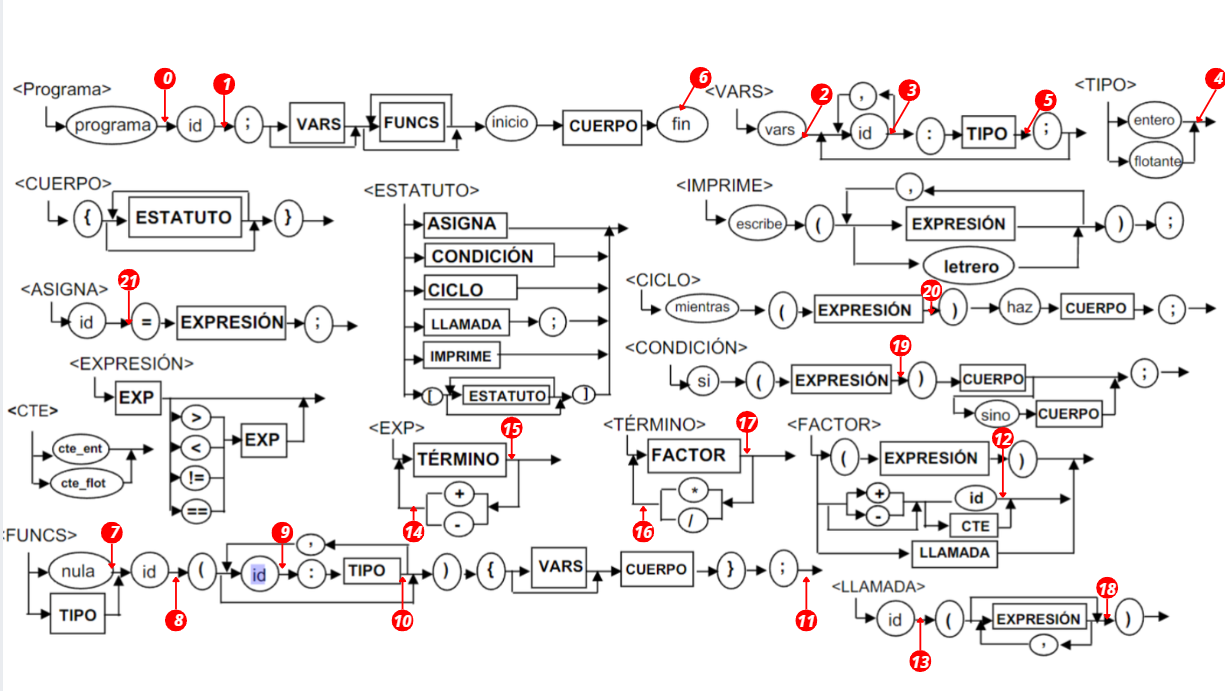
\includegraphics[width=0.8\textwidth]{image.png}
\end{figure}
\begin{longtable}{|p{1cm}|p{5.5cm}|p{4cm}|p{3cm}|}
    \caption{Puntos neurálgicos del compilador} \label{tab:puntos} \\
    \hline
    \texttt{Punto} & \texttt{Acción} & \texttt{Validación} \\
    \hline
    \endfirsthead
    \hline
    \texttt{Punto}  & \texttt{Acción} & \texttt{Validación} \\
    \hline
    \endhead
    \hline
    \endfoot
    \hline
    \endlastfoot
    %
    \texttt{P0} &
    Crear entrada en DirFun  &
    --- \\ \hline
    %

    \texttt{P1} &
    Define el nombre del programa y el scope como global &
    --- \\ \hline
    %
    \texttt{P2} &
    Si la función actual aún no tiene  VarsTable la crea y la enlaza a la función  con scope actual&
    --- \\ \hline
    %
    \texttt{P3} &
    Verifica que el \texttt{TOKEN\_ID} no exista en VarTable del scope actual 
    \break \break 
    \texttt{{{current\_id = TOKEN\_ID}}} &
    \texttt{Error:} Variable doblemente declarada \\ \hline
    %
    \texttt{P4} & 
    \texttt{{{current\_tipo = TOKEN\_TIPO}}}  &
    --- \\ \hline
    %
    \texttt{P5} & 
    Agrega 
    \break 
    \texttt{[current\_id,VAR,current\_tipo,\break global]}
    \break
    a la VarTable por cada variable declarada&
    --- \\ \hline
    %
    \texttt{P6} & 
     Cierra scope global y elimina la de VarTable local de memoria &
    --- \\ \hline
    %
    \texttt{P7} &
    \texttt{{{current\_tipo = TOKEN\_VOID}}}   &
    --- \\ \hline
    %
    \texttt{P8} & 
    Verifica que el \texttt{TOKEN\_ID} no exista en el DirFun
    \break \break
    si no existe: se agrega al DirFun con
    \break   
    \texttt{[TOKEN\_ID,  current\_tipo]}
    \break\break
    Si existe: Error  &
    \texttt{Error:} Función doblemente declarada \\ \hline
    %
    \texttt{P9} & 
    Si no existe una, crea nueva VarTable local y la asocia a la función.
    Revisa si el \texttt{TOKEN\_ID} del parametro existe en la VarTable
    \break \break
    si no: \texttt{current\_id  = TOKEN\_ID }
    \break\break
    si existe: Error &   
    \texttt{Error:} parametro doblemente declarada \\ \hline
    %
    \texttt{P10} & 
    Crea un registro en la VarTable con
    \break
    \texttt{[current\_id,PARAM,current\_tipo,\break local]} &
    --- \\ \hline
    %
    \texttt{P11} &
    Cierra el scope local ye limina VarTable local de memoria &
    --- \\ \hline
    %    
    \texttt{P12} & 
    Verifica que \texttt{TOKEN\_ID} exista en VarTable (scope local o global) &
    \texttt{Error:} Variable no declarada \\ \hline
    %    
    \texttt{P13} & 
    Verifica que \texttt{TOKEN\_ID} exista en DirFun &
    \texttt{Error:} Función no declarada \\ \hline
    %
    \texttt{P14} &
    Se agrega el operador a POper  &
    --- \\ \hline
    %
    \texttt{P15} &
    Si hay un operando (+ o - ) en POper se consultas el cubo semántico con tipos de operandos y operador &
    \texttt{Error:} Operación entre tipos incompatibles \\ \hline
    %
    \texttt{P16} &
    Se agrega el operador a POper  &
    --- \\ \hline
    %
    \texttt{P17} &
    Si hay un operando (* o / ) en POper se consultas el cubo semántico con tipos de operandos y operador &
    \texttt{Error:} Operación entre tipos incompatibles \\ \hline
    %
    \texttt{P18} &
    Verifica que los parametros tengan los tipos correctos para la función llamada&
    \texttt{Error:} Tipo de parametro inesperado \\ \hline
    %
    \texttt{P19} & 
    Verifica que el tipo de \texttt{EXPRESION} sea \texttt{BOOL} &
    \texttt{Error:} La condición debe ser de tipo booleano \\ \hline
    %
    \texttt{P20} &
    Verifica que el tipo de \texttt{EXPRESION} sea \texttt{BOOL} &
    \texttt{Error:} La condición del ciclo debe ser de tipo booleano \\ \hline
    %
    \texttt{P21} &
    Verifica que el tipo de la asignación sea compatible con el tipo de la variable &
    \texttt{Error:} Tipo incompatible \\ \hline
    %
    \texttt{P22} &
    Al encontrar \texttt{TOKEN\_RETURN}: evalúa \texttt{EXPRESION} y registra su tipo en \texttt{DirFun}. Al cerrar el scope, verifica que el tipo registrado coincida con el tipo de retorno declarado de la función. Las funciones \texttt{VOID} no pueden contener \texttt{RETURN}. &
    \texttt{Error:} Tipo de retorno incorrecto; función VOID con RETURN; función no-VOID sin RETURN \\ \hline
    %
\end{longtable}

\subsection{Justificación}

Se eligió la tabla hash para nuestras estructuras de datos ya  que las consultas en esta estructura son de costo constante ($O(1)$).


\subsection{Operaciones principales}
\begin{table}[H]
\centering
\caption{Operaciones sobre el Cubo Semántico}
\begin{tabular}{|p{4cm}|p{2cm}|p{5.5cm}|}
    \hline
    \texttt{Operación} & \texttt{Costo} & \texttt{Descripción} \\
    \hline
    \texttt{consultar(t1, t2, op)} & $O(1)$ &
    Retorna el tipo resultado de aplicar \texttt{op} entre \texttt{t1} y \texttt{t2} \\ \hline
    \texttt{esError(resultado)} & $O(1)$ &
    Verifica si el resultado es \texttt{ERROR} para lanzar
    error de tipo incompatible \\ \hline
    \texttt{operacionValida(t1, t2, op)} & $O(1)$ &
    Retorna \texttt{True} si la combinación de tipos y operador existe en el cubo \\ \hline
\end{tabular}
\end{table}

\begin{table}[H]
\centering
\caption{Operaciones sobre DirFun}
\begin{tabular}{|p{4cm}|p{2cm}|p{5.5cm}|}
    \hline
    \texttt{Operación} & \texttt{Costo} & \texttt{Descripción} \\
    \hline
    \texttt{agregar(nombre, tipo)} & $O(1)$ &
    Registra una nueva función con su tipo de retorno e inicializa su tabla de variables vacía \\ \hline
    \texttt{existe(nombre)} & $O(1)$ &
    Verifica si una función ya fue declarada. Detectar redeclaraciones \\ \hline
    \texttt{tipoRetorno(nombre)} & $O(1)$ &
    Retorna el tipo de retorno de la función \\ \hline
    \texttt{getTablaVars(nombre)} & $O(1)$ &
    Retorna la tabla de variables asociada a la función\\ \hline
\end{tabular}
\end{table}

\begin{table}[H]
\centering
\caption{Operaciones sobre VarTable}
\label{tab:ops-vartable}
\begin{tabular}{|p{4cm}|p{2cm}|p{5.5cm}|}
    \hline
    \texttt{Operación} & \texttt{Costo} & \texttt{Descripción} \\
    \hline
    \texttt{agregar(nombre, cat, tipo, scope)} & $O(1)$ &
    Registra una variable con su categoría, tipo y scope correspondiente \\ \hline
    \texttt{existe(nombre)} & $O(1)$ &
    Verifica si una variable ya fue declarada. Para detectar redeclaracione \\ \hline
    \texttt{tipo(nombre)} & $O(1)$ &
    Retorna el tipo de la variable usado como entrada al Cubo Semántico\\ \hline
    \texttt{varsEnScope(scope)} & $O(n)$ &
    Retorna todas las variables que pertenecen al scope indicado\\ \hline
    \texttt{limpiarScope(scope)} & $O(n)$ &
    Elimina todas las variables del scope indicado al salir de una función\\ \hline
\end{tabular}
\end{table}


\subsection{Definición en código}
Se agregan las definiciones de los elementos definidos anteriormente.
%
\subsubsection{Cubo Semántico}
\begin{verbatim}
    CUBO_SEMANTICO = {
        ("INT",   "INT"):   {"+": "INT",   "-": "INT",   "*": "INT",   "/": "FLOAT",
                            ">": "BOOL",  "<": "BOOL",  "!=": "BOOL", "==": "BOOL"},
        ("INT",   "FLOAT"): {"+": "FLOAT", "-": "FLOAT", "*": "FLOAT", "/": "FLOAT",
                            ">": "BOOL",  "<": "BOOL",  "!=": "BOOL", "==": "BOOL"},
        ("FLOAT", "INT"):   {"+": "FLOAT", "-": "FLOAT", "*": "FLOAT", "/": "FLOAT",
                            ">": "BOOL",  "<": "BOOL",  "!=": "BOOL", "==": "BOOL"},
        ("FLOAT", "FLOAT"): {"+": "FLOAT", "-": "FLOAT", "*": "FLOAT", "/": "FLOAT",
                            ">": "BOOL",  "<": "BOOL",  "!=": "BOOL", "==": "BOOL"},
    }
\end{verbatim}
%
\subsubsection{DirFun}
\begin{verbatim}
    DirFun {
        nombre_func -> {
            tipo_retorno : "VOID",
            tabla_vars   : TablaVariables
        }
    }
\end{verbatim}
%
\subsubsection{VarTable}
\begin{verbatim}
    VarTable {
        nombre -> {
            categoria : "VAR" | "PARAM",
            tipo      : "INT" | "FLOAT",
            scope     : "global" | nombre_funcion
        }
    }
\end{verbatim}




\section{Generación de Cudruplos}

Esta sección documenta la tercera etapa del compilador Patito la traducción del árbol sintáctico a cuádruplos. Se implementa en el módulo \texttt{patito\_cuadruplos.py}.

% ── 8.1 Estructuras de Datos ─────────────────────────────────
\subsection{Estructuras de Datos}

\subsubsection{Pilas}

La clase \texttt{Pila} es una estructura LIFO genérica.  Durante la generación de cuádruplos se instancian \texttt{tres} pilas independientes

\begin{itemize}
    \item \texttt{pila\_ops}   almacena operadores aritméticos y relacionales pendientes de procesar.
    \item \texttt{pila\_ands}  almacena operandos (nombres de variables, constantes y temporales).
    \item \texttt{pila\_tipos}almacena el tipo semántico (\texttt{INT}, \texttt{FLOAT}, \texttt{BOOL}) de cada operando en \texttt{pila\_ands}.
\end{itemize}


\subsubsection{Fila de Cuádruplos (\texttt{FilaCuadruplos})}

La clase \texttt{FilaCuadruplos} es una estructura FIFO que almacena la secuencia de cuádruplos generados.  Cada cuádruplo tiene la forma:

\[
    (\,\textit{op},\; \textit{arg1},\; \textit{arg2},\; \textit{resultado}\,)
\]

\begin{table}[H]
\centering
\caption{Operaciones de \texttt{FilaCuadruplos}}
\begin{tabular}{|p{4.5cm}|p{1.5cm}|p{6cm}|}
    \hline
    \texttt{Operación} & \texttt{Costo} & \texttt{Descripción} \\ \hline
    \texttt{agregar(op,a1,a2,res)} & $O(1)$ & Inserta el cuádruplo al final de la fila y retorna su índice \\ \hline
    \texttt{completar(idx, campo, val)} & $O(1)$ & Rellena un campo pendiente (\texttt{\_}) en el cuádruplo de índice \texttt{idx}  \\ \hline
    \texttt{siguiente()} & $O(1)$ & Retorna el índice del próximo cuádruplo a generar \\ \hline
\end{tabular}
\end{table}

% ── 8.2 Puntos Neurálgicos ───────────────────────────────────
\subsection{Puntos Neurálgicos del Generador de Cuádruplos}

A continuación se presenta cada producción gramatical relevante con sus puntos neurálgicos anotados entre corchetes \texttt{[P\_XXX]}.
\subsubsection*{Operandos}

\begin{verbatim}
factor_:  cte            [P_PUSH_OPERAND]
        | TOKEN_ID       [P_PUSH_OPERAND]
\end{verbatim}

\texttt{[P\_PUSH\_OPERAND]} Ahrega el valor del operando a \texttt{pila\_ands} y su tipo semántico (\texttt{INT} o \texttt{FLOAT}) a \texttt{pila\_tipos}.  Para \texttt{TOKEN\_ID} se consulta el directorio de funciones para obtener el tipo.

\subsubsection*{Multiplicación y División}

\begin{verbatim}
termino_: TOKEN_TIMES termino   [P_PUSH_OP_MUL -> P_GEN]
        | TOKEN_DIV   termino   [P_PUSH_OP_MUL -> P_GEN]
        | <empty>
\end{verbatim}

\texttt{[P\_PUSH\_OP\_MUL]} — Empuja \texttt{*} o \texttt{/} a \texttt{pila\_ops}, evalúa el \texttt{termino} derecho y luego dispara \texttt{[P\_GEN]}: extrae operador, dos operandos y sus tipos, consulta el cubo semántico, genera el cuádruplo \texttt{(op, izq, der, t\textit{n})} y empuja el temporal resultado.

\subsubsection*{Suma y Resta}

\begin{verbatim}
exp_: TOKEN_SUM  exp   [P_PUSH_OP_SUM -> P_GEN]
    | TOKEN_SUBS exp   [P_PUSH_OP_SUM -> P_GEN]
    | <empty>
\end{verbatim}

\texttt{[P\_PUSH\_OP\_SUM]} — Empuja \texttt{+} o \texttt{-} a \texttt{pila\_ops}, evalúa el \texttt{exp} derecho y dispara \texttt{[P\_GEN]}.

\subsubsection*{Operadores Relacionales}

\begin{verbatim}
expresion__: TOKEN_GT      exp   [P_PUSH_OP_REL -> P_GEN]
           | TOKEN_LT      exp   [P_PUSH_OP_REL -> P_GEN]
           | TOKEN_DIFF    exp   [P_PUSH_OP_REL -> P_GEN]
           | TOKEN_ISEQUAL exp   [P_PUSH_OP_REL -> P_GEN]
\end{verbatim}

\texttt{[P\_PUSH\_OP\_REL]} Agrega el operador relacional a \texttt{pila\_ops}, evalúa el \texttt{exp} derecho y dispara \texttt{[P\_GEN]}, produciendo un temporal de tipo \texttt{BOOL}.

\subsubsection*{Asignación}

\begin{verbatim}
asigna: TOKEN_ID TOKEN_EQUALS expresion TOKEN_SEMICOLON   [P_ASIGNA]
\end{verbatim}

\texttt{[P\_ASIGNA]} Evalúa \texttt{expresion}, extrae el resultado de \texttt{pila\_ands} y genera el cuádruplo \texttt{(=, resultado, \_, var)}.

\subsubsection*{Impresión}

\begin{verbatim}
imprime_: expresion  imprime__   [P_PRINT]
        | TOKEN_LETRERO imprime__ [P_PRINT_LETRERO]
\end{verbatim}

\texttt{[P\_PRINT]} Evalúa la expresión, extrae el resultado y genera \texttt{(PRINT, resultado, \_, \_)}.\\
\texttt{[P\_PRINT\_LETRERO]} Genera directamente \texttt{(PRINT, "letrero", \_, \_)} sin evaluar expresión.

\subsubsection*{Condicional }

\begin{verbatim}
condicion:
  TOKEN_IF TOKEN_LPAREN
    expresion                  [P_IF_COND]
  TOKEN_RPAREN                 [P_GOTOF]
    cuerpo                     [P_IF_BODY]
    condicion_                 [P_GOTO? / P_FILL_IF]
  TOKEN_SEMICOLON

condicion_: TOKEN_ELSE cuerpo  [P_ELSE_BODY / P_FILL_ELSE]
          | <empty>
\end{verbatim}

\begin{itemize}
    \item \texttt{[P\_IF\_COND]} Evalúa la expresión booleana de la condición.
    \item \texttt{[P\_GOTOF]} Genera \texttt{(GOTOF, cond, \_, \_)} con destino pendiente.
    \item \texttt{[P\_IF\_BODY]} Genera los cuádruplos del bloque \texttt{IF}.
    \item \texttt{[P\_GOTO]} Si existe \texttt{ELSE}: genera \texttt{(GOTO, \_, \_, \_)} con destino pendiente para saltar el bloque \texttt{ELSE}.
    \item \texttt{[P\_FILL\_IF]} Rellena el destino del \texttt{GOTOF} con la posición actual.
    \item \texttt{[P\_ELSE\_BODY]} Genera los cuádruplos del bloque \texttt{ELSE}.
    \item \texttt{[P\_FILL\_ELSE]} Rellena el destino del \texttt{GOTO} con la posición actual.
\end{itemize}

\subsubsection*{Ciclo }

\begin{verbatim}
ciclo:
  TOKEN_WHILE               [P_WHILE_START]
  TOKEN_LPAREN
    expresion               [P_WHILE_COND]
  TOKEN_RPAREN              [P_GOTOF]
  TOKEN_DO
    cuerpo                  [P_WHILE_BODY]
                            [P_GOTO_BACK]
                            [P_FILL_WHILE]
  TOKEN_SEMICOLON
\end{verbatim}

\begin{itemize}
    \item \texttt{[P\_WHILE\_START]} Guarda el índice actual de la fila como \texttt{pos\_inicio} (punto de regreso del ciclo).
    \item \texttt{[P\_WHILE\_COND]} Evalúa la expresión booleana de la condición del ciclo.
    \item \texttt{[P\_GOTOF]} Genera \texttt{(GOTOF, cond, \_, \_)} con destino pendiente.
    \item \texttt{[P\_WHILE\_BODY]} Genera los cuádruplos del cuerpo del ciclo.
    \item \texttt{[P\_GOTO\_BACK]} Genera \texttt{(GOTO, \_, \_, pos\_inicio)} para regresar al inicio del ciclo.
    \item \texttt{[P\_FILL\_WHILE]} Rellena el destino del \texttt{GOTOF} con la posición actual (salida del ciclo).
\end{itemize}

\subsubsection*{Llamada a función}

\begin{verbatim}
llamada: TOKEN_ID TOKEN_LPAREN llamada_ TOKEN_RPAREN   [P_CALL]

llamada_:  expresion llamada__   [P_PARAM]
         | <empty>
\end{verbatim}

\texttt{[P\_PARAM]} Por cada argumento evaluado genera \texttt{(PARAM, arg, \_, \_)}.\\
\texttt{[P\_CALL]} Verifica que la función exista en \texttt{DirFun} y genera \texttt{(CALL, nombre\_func, \_, t\textit{n})}, además verifica que los parametros sean del tipo y cantidad correcta. \\
\texttt{[P\_RETURN]} Verifica que el valor de retorno sea del tipo correcto y genera \texttt{(RETURN, val, \_, \_)}. \\
% ── 8.3 Tabla resumen ────────────────────────────────────────
\subsection{Tabla de Puntos Neurálgicos}

\begin{longtable}{|p{4.2cm}|p{5cm}|p{5.5cm}|}
    \caption{Puntos neurálgicos del generador de cuádruplos} \\
    \hline
    \texttt{Punto} & \texttt{Acción} & \texttt{Cuádruplo generado} \\
    \hline
    \endfirsthead
    \hline
    \texttt{Punto} & \texttt{Acción} & \texttt{Cuádruplo generado} \\
    \hline
    \endhead
    \hline
    \endfoot
    \hline
    \endlastfoot
    %
    \texttt{P\_PUSH\_OPERAND} &
    Agrega operando y tipo a \texttt{pila\_ands}/\texttt{pila\_tipos} &
    --- \\ \hline
    %
    \texttt{P\_PUSH\_OP\_MUL} &
    Agrega \texttt{*} o \texttt{/} a \texttt{pila\_ops} &
    --- \\ \hline
    %
    \texttt{P\_PUSH\_OP\_SUM} &
    Agrega \texttt{+} o \texttt{-} a \texttt{pila\_ops} &
    --- \\ \hline
    %
    \texttt{P\_PUSH\_OP\_REL} &
    Agrega operador relacional a \texttt{pila\_ops} &
    --- \\ \hline
    %
    \texttt{P\_GEN} &
    Pop operador + 2 operandos, consulta cubo semántico, genera cuádruplo, empuja temporal &
    \texttt{(op, izq, der, t\textit{n})} \\ \hline
    %
    \texttt{P\_ASIGNA} &
    Pop resultado de \texttt{pila\_ands}, genera cuádruplo de asignación &
    \texttt{(=, val, \_, var)} \\ \hline
    %
    \texttt{P\_PRINT} &
    Pop resultado o letrero, genera cuádruplo de impresión &
    \texttt{(PRINT, val, \_, \_)} \\ \hline
    %
    \texttt{P\_IF\_COND} &
    Evalúa expresión booleana del IF &
    --- \\ \hline
    %
    \texttt{P\_GOTOF} &
    Genera salto condicional con destino pendiente &
    \texttt{(GOTOF, cond, \_, ?)} \\ \hline
    %
    \texttt{P\_GOTO} &
    Genera salto incondicional con destino pendiente (fin del IF) &
    \texttt{(GOTO, \_, \_, ?)} \\ \hline
    %
    \texttt{P\_FILL\_IF} &
    Rellena destino del GOTOF &
    --- \\ \hline
    %
    \texttt{P\_FILL\_ELSE} &
    Rellena destino del GOTO &
    --- \\ \hline
    %
    \texttt{P\_WHILE\_START} &
    Guarda \texttt{pos\_inicio} de la fila &
    --- \\ \hline
    %
    \texttt{P\_GOTO\_BACK} &
    Genera salto de regreso al inicio del ciclo &
    \texttt{(GOTO, \_, \_, pos\_inicio)} \\ \hline
    %
    \texttt{P\_FILL\_WHILE} &
    Rellena destino del GOTOF del ciclo &
    --- \\ \hline
    %
    \texttt{P\_PARAM} &
    Genera cuádruplo de parámetro para la llamada &
    \texttt{(PARAM, arg, \_, \_)} \\ \hline
    %
    \texttt{P\_CALL} &
    Verifica existencia de la función. Genera cuádruplo de llamada &
    \texttt{(CALL, func, \_, t\textit{n})} \\ \hline
    \texttt{P\_RETURN} &
    Verifica que el valor de retorno sea del tipo correcto &
    \texttt{(RETURN, val, \_,\_)} \\ \hline
    
\end{longtable}

% ── 8.4 Resultados de casos de prueba ────────────────────────
\subsection{Resultados de Casos de Prueba}

A continuación se presentan los cuádruplos generados por \texttt{patito\_cuadruplos.py} para cada caso de prueba.


\subsubsection*{TEST 1. Expresiones aritméticas}

Programa con asignaciones enteras y expresión \texttt{a + b * 2}.  La multiplicación se resuelve primero (mayor precedencia) produciendo el temporal \texttt{t1}, luego la suma produce \texttt{t2}.

\begin{verbatim}
#     Op         Arg1            Arg2            Resultado
----------------------------------------------------------
0     =          5               _               a
1     =          3               _               b
2     *          b               2               t1
3     +          a               t1              t2
4     =          t2              _               c
5     PRINT      c               _               _
\end{verbatim}

\subsubsection*{TEST 2. Flotantes y PRINT con letrero}

Programa con variables \texttt{FLOAT} y \texttt{PRINT} de letrero seguido de expresión.  Los literales flotantes \texttt{2.0} y \texttt{1.0} se reconocen como tipo \texttt{FLOAT} en el cubo semántico.

\begin{verbatim}
#     Op         Arg1            Arg2            Resultado
----------------------------------------------------------
0     =          4               _               n
1     =          3.14            _               x
2     *          x               2.0             t1
3     +          t1              1.0             t2
4     =          t2              _               x
5     PRINT      "Resultado: "   _               _
6     PRINT      x               _               _
\end{verbatim}

\subsubsection*{TEST 3. Condicional IF-ELSE}

El cuádruplo \texttt{GOTOF} (índice 3) salta al cuádruplo 6 (inicio del ELSE) si la condición es falsa.  El \texttt{GOTO} (índice 5) salta al cuádruplo 7 para omitir el bloque ELSE cuando la condición fue verdadera.

\begin{verbatim}
#     Op         Arg1            Arg2            Resultado
----------------------------------------------------------
0     =          10              _               a
1     =          5               _               b
2     >          a               b               t1
3     GOTOF      t1              _               6
4     PRINT      "a es mayor"    _               _
5     GOTO       _               _               7
6     PRINT      "b es mayor o igual" _          _
\end{verbatim}

\subsubsection*{TEST 4. Ciclo WHILE}

\texttt{P\_WHILE\_START} guarda \texttt{pos\_inicio = 2} (cuádruplo de la condición).  El \texttt{GOTOF} en el índice 3 salta al cuádruplo 9 (salida del ciclo) cuando \texttt{i >= 6}.  El \texttt{GOTO} en el índice 8 retrocede al cuádruplo 2 para reevaluar la condición.

\begin{verbatim}
#     Op         Arg1            Arg2            Resultado
----------------------------------------------------------
0     =          1               _               i
1     =          0               _               suma
2     <          i               6               t1
3     GOTOF      t1              _               9
4     +          suma            i               t2
5     =          t2              _               suma
6     +          i               1               t3
7     =          t3              _               i
8     GOTO       _               _               2
9     PRINT      suma            _               _
\end{verbatim}

\subsubsection*{TEST 5. Función y llamada}

Los cuádruplos 0--2 corresponden al cuerpo de la función \texttt{calcular}.  Los cuádruplos 3--6 corresponden al cuerpo principal: asignaciones de \texttt{a} y \texttt{b}, dos cuádruplos \texttt{PARAM} para los argumentos, y el \texttt{CALL} a \texttt{calcular}.

\begin{verbatim}
#     Op         Arg1            Arg2            Resultado
----------------------------------------------------------
0     +          x               y               t1
1     =          t1              _               temp
2     PRINT      temp            _               _
3     =          3               _               a
4     =          4               _               b
5     PARAM      a               _               _
6     PARAM      b               _               _
7     CALL       calcular        _               t2
\end{verbatim}

\section{Direcciones de memoria virtual}
A continuación se documenta la distribución de las direcciones virtuales, para la cual se opto por bloques reservados para cada tipo de dato y scope.
\begin{table}[H]
\centering
\caption{Direcciones virtuales}
\label{tab:cubo}
\begin{tabular}{|c|c|c|c|}
    \hline
    \texttt{Scope} & \texttt{Tipo} & \texttt{Inicio} & \texttt{Fin} \\
    \hline
    % GLOBALES
    \texttt{Global}   & \texttt{INT}   & \texttt{1000} & \texttt{1099}   \\ \hline
    \texttt{Global}   & \texttt{FLOAT} & \texttt{1100} & \texttt{1199}   \\ \hline
    \texttt{Global}   & \texttt{BOOL} & \texttt{1200} & \texttt{1299}   \\ \hline
    \texttt{Local}   & \texttt{INT}   & \texttt{2000} & \texttt{2099}   \\ \hline
    \texttt{Local}   & \texttt{FLOAT} & \texttt{2100} & \texttt{2199}   \\ \hline
    \texttt{Local}   & \texttt{BOOL} & \texttt{2200} & \texttt{2299}   \\ \hline
    \texttt{Param}   & \texttt{INT}   & \texttt{3000} & \texttt{3099}   \\ \hline
    \texttt{Param}   & \texttt{FLOAT} & \texttt{3100} & \texttt{3199}   \\ \hline
    \texttt{Param}   & \texttt{BOOL} & \texttt{3200} & \texttt{3299}   \\ \hline
    \texttt{Temp}   & \texttt{INT}   & \texttt{4000} & \texttt{4099}   \\ \hline
    \texttt{Temp}   & \texttt{FLOAT} & \texttt{4100} & \texttt{4199}   \\ \hline
    \texttt{Temp}   & \texttt{BOOL} & \texttt{4200} & \texttt{4299}   \\ \hline
    \texttt{Const} & \texttt{INT}   & \texttt{5000} & \texttt{5099}   \\ \hline
    \texttt{Const} & \texttt{FLOAT} & \texttt{5100} & \texttt{5199}   \\ \hline
    \texttt{Const} & \texttt{BOOL} & \texttt{5200} & \texttt{5299}   \\ \hline
\end{tabular}
\end{table}

% ============================================================
\section{Máquina Virtual}
% ============================================================

La Máquina Virtual de Patitoc interpreta la lista de cuádruplos generada por el compilador. Su arquitectura consta de tres estructuras principales: \texttt{MemoriaEjecucion}, \texttt{RegistroActivacion} y \texttt{MaquinaVirtual}.

% ── 11.1 MemoriaEjecucion ────────────────────────────────────
\subsection{Estructura: \texttt{MemoriaEjecucion}}

\subsubsection*{Descripción}

\texttt{MemoriaEjecucion} es una memoria de ejecución \emph{plana} implementada sobre un diccionario Python \texttt{\_mem: dict[int, object]}. Cada dirección virtual, asignada en tiempo de compilación, es la clave entera; su valor es el dato en tiempo de ejecución. La clase define cinco segmentos lógicos identificados exclusivamente por el rango numérico de la dirección.

\begin{table}[H]
\centering
\caption{Segmentos lógicos de \texttt{MemoriaEjecucion}}
\label{tab:segmentos-mem}
\begin{tabular}{|c|c|l|}
    \hline
    \texttt{Segmento} & \texttt{Rango} & \texttt{Contenido} \\ \hline
    \texttt{global} & 1000--1999 & Variables globales del programa \\ \hline
    \texttt{local}  & 2000--2999 & Variables locales de funciones  \\ \hline
    \texttt{param}  & 3000--3999 & Parámetros de funciones         \\ \hline
    \texttt{temp}   & 4000--4999 & Temporales del compilador       \\ \hline
    \texttt{const}  & 5000--5999 & Constantes literales (solo lectura) \\ \hline
\end{tabular}
\end{table}

\subsubsection*{Versión gráfica}
 
\begin{table}[H]
\centering
\caption{Mapa de la \texttt{MemoriaEjecucion} y ejemplo de estado}
\label{tab:memejecucion}
\begin{tabular}{|c|c|l||c|c|}
    \hline
    \multicolumn{3}{|c||}{\textbf{Espacio de Direcciones}} &
    \multicolumn{2}{c|}{\textbf{Snapshot en ejecución}} \\
    \hline
    \textbf{Rango} & \textbf{Segmento} & \textbf{Contenido típico} &
    \textbf{Addr} & \textbf{\_mem{[}addr{]}} \\ \hline
    \colorbox{green!20}{1000--1999}  & \texttt{global} & INT/FLOAT/BOOL globales & 1000 & 10   \\ \hline
    \colorbox{blue!15}{2000--2999}   & \texttt{local}  & INT/FLOAT/BOOL locales  & 2000 & 7    \\ \hline
    \colorbox{orange!20}{3000--3999} & \texttt{param}  & Parámetros de función   & 3000 & 3    \\ \hline
    \colorbox{yellow!30}{4000--4999} & \texttt{temp}   & Temporales BOOL/INT/FLT & 4200 & True \\ \hline
    \colorbox{gray!20}{5000--5999}   & \texttt{const}  & Literales (read-only)   & 5000 & 10   \\ \hline
\end{tabular}
\end{table}

El diccionario interno en un momento concreto de ejecución luce así:

\begin{verbatim}
_mem = {
    1000: 10,     # variable 'a', INT global
    1001:  5,     # variable 'b', INT global
    3000:  3,     # parámetro 'x', INT
    4200: True,   # temporal t1, BOOL
    5000: 10,     # constante literal 10
    5001:  5,     # constante literal 5
}
\end{verbatim}

\subsubsection*{Métodos de acceso principales}

\begin{table}[H]
\centering
\caption{Métodos de \texttt{MemoriaEjecucion}}
\label{tab:metodos-mem}
\begin{tabular}{|p{3.8cm}|p{1.5cm}|p{7.7cm}|}
    \hline
    \texttt{Método} & \texttt{Costo} & \texttt{Descripción} \\ \hline
    \texttt{segmento(addr)} & $O(1)$ &
    Recorre la lista de 5 segmentos y retorna el nombre del segmento al que pertenece \texttt{addr}. Lanza \texttt{RuntimeError} si la dirección está fuera de rango. \\ \hline
    \texttt{leer(addr)} & $O(1)$ &
    Valida el rango y retorna \texttt{\_mem.get(addr, 0)}.  \\ \hline
    \texttt{escribir(addr, valor)} & $O(1)$ &
    Verifica que \texttt{addr} no pertenezca al segmento \texttt{const} (protección de solo lectura) y actualiza \texttt{\_mem[addr]}. \\ \hline
    \texttt{precargar(addr, valor)} & $O(1)$ &
    Carga constantes literales sin validar el segmento; invocado una sola vez al construir \texttt{MaquinaVirtual}. \\ \hline
    \texttt{dump()} & $O(n)$ &
    Retorna una cadena de depuración con todas las entradas del diccionario ordenadas por dirección, indicando su segmento. \\ \hline
\end{tabular}
\end{table}

% ── 11.2 RegistroActivacion ──────────────────────────────────
\subsection{Estructura: \texttt{RegistroActivacion}}

\subsubsection*{Descripción}

Cada llamada a función empuja un \texttt{RegistroActivacion} sobre la pila de llamadas de \texttt{MaquinaVirtual}. El registro almacena el estado mínimo necesario para restaurar la ejecución al retornar.

\subsubsection*{Versión gráfica}

El siguiente esquema muestra el estado de la pila durante la ejecución de \texttt{fib(2)} (Fibonacci recursivo), donde tres frames están activos simultáneamente:

\begin{table}[H]
\centering
\caption{Estado de la pila de llamadas durante \texttt{fib(2)}}
\label{tab:pila-activacion}
\begin{tabular}{|c|c|c|c|p{4cm}|}
    \hline
    \textbf{Frame} & \texttt{nombre} & \texttt{retorno\_ip} & \texttt{retorno\_dir} & \texttt{snapshot} \\ \hline
    tope (3er) & \texttt{"fib"} & 12 & 4003 & \{2000:0, 2001:1\} \\ \hline
    2do        & \texttt{"fib"} & 12 & 4001 & \{2000:0, 2001:0\} \\ \hline
    base (1er) & \texttt{"fib"} & 23 & 4005 & \{\}              \\ \hline
\end{tabular}
\end{table}

\subsubsection*{Campos}

\begin{table}[H]
\centering
\caption{Campos de \texttt{RegistroActivacion}}
\label{tab:registro-activacion}
\begin{tabular}{|p{3.2cm}|p{2.8cm}|p{7cm}|}
    \hline
    \texttt{Campo} & \texttt{Tipo} & \texttt{Descripción} \\ \hline
    \texttt{nombre} & \texttt{str} &
    Nombre de la función llamada. Usado para mensajes de error y depuración. \\ \hline
    \texttt{retorno\_ip} & \texttt{int} &
    Índice del cuádruplo al que retorna la ejecución después de \texttt{ENDPROC} o \texttt{RETURN}. Equivale a \texttt{ip + 1} del cuádruplo \texttt{CALL}. \\ \hline
    \texttt{retorno\_dir} & \texttt{int | None} &
    Dirección virtual donde se almacena el valor de retorno. Es \texttt{None} para funciones \texttt{VOID}. \\ \hline
    \texttt{snapshot} & \texttt{dict} &
    Captura de los valores actuales de locales y parámetros tomada \emph{antes} de sobrescribirlos con los de la nueva llamada. Se restaura con \texttt{\_mem.update(snapshot)} al retornar, habilitando la recursión. \\ \hline
\end{tabular}
\end{table}

% ── 11.3 MaquinaVirtual ──────────────────────────────────────
\subsection{Estructura: \texttt{MaquinaVirtual}}

\subsubsection*{Descripción}

\texttt{MaquinaVirtual} es el ejecutor de cuádruplos. Mantiene un puntero de instrucción \texttt{ip} e itera sobre la lista de cuádruplos invocando \texttt{\_despachar(op, arg1, arg2, res)} en cada paso.

\subsubsection*{Atributos principales}

\begin{table}[H]
\centering
\caption{Atributos de \texttt{MaquinaVirtual}}
\label{tab:mv-atributos}
\begin{tabular}{|p{3.5cm}|p{3.5cm}|p{6cm}|}
    \hline
    \texttt{Atributo} & \texttt{Tipo} & \texttt{Descripción} \\ \hline
    \texttt{cuadruplos} & \texttt{list[tuple]} &
    Lista de cuádruplos \texttt{(op,\,arg1,\,arg2,\,res)} producidos por el compilador. \\ \hline
    \texttt{memoria} & \texttt{MemoriaEjecucion} &
    Almacén plano de variables, parámetros, temporales y constantes. \\ \hline
    \texttt{pila\_llamadas} & \texttt{list[Registro\-Activacion]} &
    Pila de frames activos; crece con \texttt{CALL} y decrece con \texttt{RETURN}/\texttt{ENDPROC}. \\ \hline
    \texttt{pila\_params} & \texttt{list} &
    Staging de argumentos: los valores evaluados por cuádruplos \texttt{PARAM} se acumulan aquí hasta el siguiente \texttt{CALL}. \\ \hline
    \texttt{ip} & \texttt{int} &
    Puntero de instrucción; índice del cuádruplo en ejecución. \\ \hline
\end{tabular}
\end{table}

\subsubsection*{Ciclo de ejecución}

\begin{verbatim}
def ejecutar(self) -> None:
    self.ip = 0
    while self.ip < len(self.cuadruplos):
        op, arg1, arg2, res = self.cuadruplos[self.ip]
        self._despachar(op, arg1, arg2, res)
\end{verbatim}

Los opcodes soportados son: \texttt{=}, \texttt{+}, \texttt{-}, \texttt{*}, \texttt{/}, \texttt{NEG}, \texttt{>}, \texttt{<}, \texttt{!=}, \texttt{==}, \texttt{PRINT}, \texttt{GOTO}, \texttt{GOTOF}, \texttt{PARAM}, \texttt{CALL}, \texttt{RETURN}, \texttt{ENDPROC}, \texttt{END}.

% ── 11.4 Direcciones Virtuales ───────────────────────────────
\subsection{Cómo las Direcciones Virtuales Indexan la Memoria}

El compilador asigna a cada símbolo una dirección virtual única en tiempo de compilación. Esta dirección es el único dato que la MV necesita para acceder a la memoria en tiempo de ejecución.

\begin{enumerate}
    \item \textbf{Identificación de segmento sin metadato extra.}
    El rango numérico de la dirección identifica el segmento de forma fácil:
    $1000{-}1999 : \texttt{global}$,
    $2000{-}2999 : \texttt{local}$,
    $3000{-}3999 : \texttt{param}$,
    $4000{-}4999 : \texttt{temp}$,
    $5000{-}5999 : \texttt{const}$.

    \item \textbf{Acceso en $O(1)$ sin búsqueda por nombre.}
    Los cuádruplos contienen direcciones enteras  en lugar de nombres (\texttt{a}, \texttt{t1}). La MV ejecuta \texttt{\_mem[addr]} directamente, sin consultar el Directorio de Funciones ni la Tabla de Variables

    \item \textbf{Constantes precargadas al iniciar.}
    Al construir \texttt{MaquinaVirtual}, todas las constantes literales registradas en \texttt{MemoriaVirtual} se copian al diccionario vía \texttt{precargar}, ocupando el segmento \texttt{const}

    \item \textbf{Recursión habilitada por \texttt{snapshot}.}
    Las direcciones de locales y parámetros son únicas globalmente, por lo que llamadas recursivas sobrescribirían los valores de la invocación padre. Cada \texttt{RegistroActivacion} captura un \texttt{snapshot} antes de sobrescribir y lo restaura al retornar, logrando el efecto de un frame por invocación.
\end{enumerate}

\begin{table}[H]
\centering
\caption{Ejemplo de traducción nombre $\rightarrow$ dirección virtual $\rightarrow$ clave en \texttt{\_mem}}
\label{tab:traduccion-dirs}
\begin{tabular}{|p{3.5cm}|p{1.8cm}|p{2cm}|p{2cm}|p{3.3cm}|}
    \hline
    \texttt{Símbolo} & \texttt{Categoría} & \texttt{Segmento} & \texttt{Dirección} & \texttt{En \_mem} \\ \hline
    \texttt{a} (global INT)   & VAR   & global & 1000 & \texttt{\_mem[1000] = 10}   \\ \hline
    \texttt{b} (global INT)   & VAR   & global & 1001 & \texttt{\_mem[1001] = 5}    \\ \hline
    \texttt{x} (param INT)    & PARAM & param  & 3000 & \texttt{\_mem[3000] = 3}    \\ \hline
    \texttt{t1} (BOOL temp)   & TEMP  & temp   & 4200 & \texttt{\_mem[4200] = True} \\ \hline
    \texttt{``10''} (const INT) & CONST & const  & 5000 & \texttt{\_mem[5000] = 10}   \\ \hline
\end{tabular}
\end{table}

% ── 11.5 Casos de Prueba ─────────────────────────────────────
\subsection{Casos de Prueba de la Máquina Virtual}

A continuación se presentan los programas de prueba, sus cuádruplos reales con direcciones virtuales y la salida producida por la MV.

% ── TEST 2 ───────────────────────────────────────────────────
\subsubsection*{TEST 2 --- Flotantes y \texttt{PRINT} con letrero}


\begin{verbatim}
PROGRAM prog2 ;
VARS x : FLOAT ; n : INT ;
BEGIN {
    n = 4 ;
    x = 3.14 ;
    x = x * 2.0 + 1.0 ;
    PRINT( "Resultado: " , x ) ;
} END
\end{verbatim}

Cuádruplos generados (con direcciones virtuales):
\begin{verbatim}
#   Op      Arg1   Arg2   Res    Nota
--  ------  -----  -----  -----  --------------------------------
0   GOTO    _      _      1
1   =       5000   _      1000   n  = const(4)
2   =       5100   _      1100   x  = const(3.14)
3   *       1100   5101   4100   t1 = x * const(2.0)
4   +       4100   5102   4101   t2 = t1 + const(1.0)
5   =       4101   _      1100   x  = t2
6   PRINT   5300   _      _      imprime "Resultado: "
7   PRINT   1100   _      _      imprime x
8   END     _      _      _
\end{verbatim}

Salida:
\begin{verbatim}
Resultado:
7.28
\end{verbatim}

% ── TEST 3 ───────────────────────────────────────────────────
\subsubsection*{TEST 3 --- Condicional \texttt{IF-ELSE}}


\begin{verbatim}
PROGRAM prog3 ;
VARS a, b : INT ;
BEGIN {
    a = 10 ; b = 5 ;
    IF ( a > b ) { PRINT( "a es mayor" ) ; }
    ELSE         { PRINT( "b es mayor o igual" ) ; } ;
} END
\end{verbatim}

\begin{verbatim}
#   Op      Arg1   Arg2   Res    Nota
--  ------  -----  -----  ---  ------------------------------------
0   GOTO    _      _      1
1   =       5000   _      1000  a = 10
2   =       5001   _      1001  b = 5
3   >       1000   1001   4200  t1 = a > b
4   GOTOF   4200   _      7     si t1=False, salta al bloque ELSE
5   PRINT   5300   _      _     "a es mayor"
6   GOTO    _      _      8     salta el bloque ELSE
7   PRINT   5301   _      _     "b es mayor o igual"
8   END     _      _      _
\end{verbatim}

Salida:
\begin{verbatim}
a es mayor
\end{verbatim}

% ── TEST 4 ───────────────────────────────────────────────────
\subsubsection*{TEST 4 --- Ciclo \texttt{WHILE}}


\begin{verbatim}
PROGRAM prog4 ;
VARS i, suma : INT ;
BEGIN {
    i = 1 ; suma = 0 ;
    WHILE ( i < 6 ) DO {
        suma = suma + i ;
        i = i + 1 ;
    } ;
    PRINT( suma ) ;
} END
\end{verbatim}

Cuádruplos generados:
\begin{verbatim}
#   Op      Arg1   Arg2   Res    Nota
--  ------  -----  -----  ---  ------------------------------------
0   GOTO    _      _      1
1   =       5000   _      1000  i    = 1
2   =       5001   _      1001  suma = 0
3   <       1000   5002   4200  t1   = i < 6
4   GOTOF   4200   _      10    si t1=False, sale del ciclo
5   +       1001   1000   4000  t2   = suma + i
6   =       4000   _      1001  suma = t2
7   +       1000   5000   4001  t3   = i + 1
8   =       4001   _      1000  i    = t3
9   GOTO    _      _      3     regresa a evaluar la condición
10  PRINT   1001   _      _     imprime suma
11  END     _      _      _
\end{verbatim}

Salida:
\begin{verbatim}
15
\end{verbatim}

% ── TEST 6 ───────────────────────────────────────────────────
\subsubsection*{TEST 6 --- Fibonacci Iterativo}


\begin{verbatim}
PROGRAM fibonacci ;
VARS r : INT ;
INT fib ( num : INT ) {
    VARS a, b, temp, i : INT ;
    {
        a = 0 ; b = 1 ; i = 0 ;
        WHILE ( i < num ) DO {
            temp = a + b ; a = b ; b = temp ; i = i + 1 ;
        } ;
    }
    RETURN a ;
} ;
BEGIN {
    PRINT( "fib(0):" ) ; r = fib( 0 ) ; PRINT( r ) ;
    PRINT( "fib(5):" ) ; r = fib( 5 ) ; PRINT( r ) ;
    PRINT( "fib(10):" ) ; r = fib( 10 ) ; PRINT( r ) ;
} END
\end{verbatim}

Salida:
\begin{verbatim}
fib(0):
0
fib(5):
5
fib(10):
55
\end{verbatim}

% ── TEST 7 ───────────────────────────────────────────────────
\subsubsection*{TEST 7 --- Fibonacci Recursivo}

\begin{verbatim}
PROGRAM fibonacci_recursivo ;
VARS r : INT ;
INT fib ( n : INT ) {
    VARS a, b : INT ;
    {
        IF ( n == 0 ) { a = 0 ; } ELSE {
            IF ( n == 1 ) { a = 1 ; } ELSE {
                a = fib( n - 1 ) ;
                b = fib( n - 2 ) ;
                a = a + b ;
            } ;
        } ;
    }
    RETURN a ;
} ;
BEGIN {
    PRINT( "fib(0):" ) ; r = fib( 0 ) ; PRINT( r ) ;
    PRINT( "fib(5):" ) ; r = fib( 5 ) ; PRINT( r ) ;
    PRINT( "fib(10):" ) ; r = fib( 10 ) ; PRINT( r ) ;
} END
\end{verbatim}

Salida:
\begin{verbatim}
fib(0):
0
fib(5):
5
fib(10):
55
\end{verbatim}

% ── TEST 8 ───────────────────────────────────────────────────
\subsubsection*{TEST 8 --- Factorial Recursivo}

\begin{verbatim}
PROGRAM factorial ;
VARS r : INT ;
INT fact ( n : INT ) {
    VARS res : INT ;
    {
        IF ( n == 0 ) { res = 1 ; } ELSE {
            res = n * fact( n - 1 ) ;
        } ;
    }
    RETURN res ;
} ;
BEGIN {
    PRINT( "fact(0):" ) ; r = fact( 0 ) ; PRINT( r ) ;
    PRINT( "fact(5):" ) ; r = fact( 5 ) ; PRINT( r ) ;
    PRINT( "fact(10):" ) ; r = fact( 10 ) ; PRINT( r ) ;
} END
\end{verbatim}

Salida:
\begin{verbatim}
fact(0):
1
fact(5):
120
fact(10):
3628800
\end{verbatim}


\section*{Declaración de Uso de Inteligencia Artificial}

El presente documento fue elaborado con apoyo de la herramienta de
inteligencia artificial Claude (Anthropic) como asistente en la
redacción y estructuración del contenido en \LaTeX.

Las actividades en las que se utilizó la herramienta fueron:

\begin{itemize}
    \item Generación y corrección de la plantilla base en \LaTeX\
          compatible con MiKTeX y LaTeX Workshop. 
    \item Implementación de estructuras de datos básica del cubo semántico, Directorio de Funciones y
          Tablas de Variables.
    \item Generación del código en Python que implementa estructuras básicas
          de pilas y filas.
    \item Elaboración de las tablas de métodos de acceso y casos de prueba.
\end{itemize}

Todas las decisiones de diseño, definición de tokens, gramática
y validaciones semánticas y documentación fueron revisadas y aprobadas por el
autor, quien es responsable del contenido final del documento.

\vspace{1cm}
\noindent
\begin{tabular}{@{}p{6cm}@{}}
    \hline \\[-0.8em]
    Carlos Fernando Ramos Mena \\
    Matrícula: A01197622 \\
    \today
\end{tabular}
\end{document}

